%%%%%%%%%%%%%%%%%%%%%%%%%%%%%%%%%%%%%%%%%
%
% Space Physics
% Practical 2B
% git cola
%%%%%%%%%%%%%%%%%%%%%%%%%%%%%%%%%%%%%%%%%

%----------------------------------------------------------------------------------------
%	DOCUMENT CONFIGURATIONS
%----------------------------------------------------------------------------------------

\documentclass{article}

\title{\textbf {Space Physics} \\ Practical 2B\\ Data Analysis\\ Revision 2} % Title
\def\authorivan{Ivan \v Sinkarenko}
\def\authoranu{Anuraj Rajendraprakash}
\author{\authorivan\\\authoranu}

\usepackage{graphicx}
\usepackage{fullpage}
\usepackage{url}
\usepackage{color}

% load package with ``framed'' and ``numbered'' option.
\usepackage[framed,numbered,autolinebreaks,useliterate]{mcode}

\begin{document}

\maketitle % Insert the title, author and date

\centerline{Referee: Gabriella Stenberg}

\setlength\parindent{0pt} % Removes all indentation from paragraphs

\renewcommand{\labelenumi}{\alph{enumi}} % Make numbering in the enumerate environment by letter rather than number
\clearpage

\tableofcontents

\listoffigures

\clearpage

%----------------------------------------------------------------------------------------
%	SECTION 1. Time Series Data
%----------------------------------------------------------------------------------------
\section{Time Series Data}

\subsection{Question 1}
\textit{Where in the magnetosphere are the observations made? Motivate you
answer!}

The measurment taken on 2002-03-02 at 03:29-03:30 is taken at the time when the satellite was crossing the border of magnetopause.

\begin{figure}[htb!]
\centering
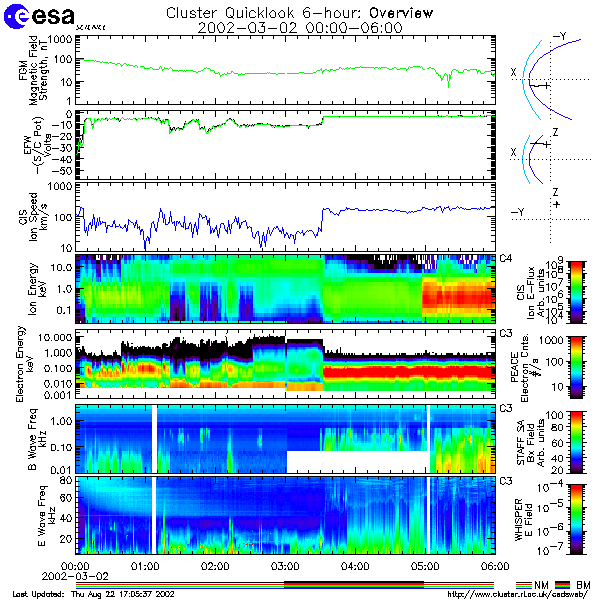
\includegraphics[width=0.7\textwidth]{Figures/cluster.png}
\caption{Cluster Quicklook 6-hours overview.}
\label{fig:cluster}
\end{figure}

\subsection{Question 2}
\textit{Plot the time series (all components) from the three instruments. Can you identify any waves? What type of waves are we looking at: Electrostatic or electromagnetic? Is there a need to correct the data somehow? If so, why and how do you do that?}

Electromagnetic between 20 and 30 s. Electrostatic between 55 and 60 s. x component is facing towards the sun. It should fluctuate around zero, like the y-component does it. It happens because of the photon emission, which is captured by the probes. There is an oscillation with constant frequency and a DC shift in the x component of the electric field. These effects are common in a double probe measurement on board a spinning spacecraft. The constant oscillation seen in Figure \ref{fig:EFW} is due to the spin of the spacecraft, this oscillation has half the rotation period of the spacecraft, which is approximately 2 seconds for the given data. For using the data properly these effects have to be removed from the data. The DC shift can be removed by taking the average of the data and then subtracting it. For removing the oscillations from the data signal processing can be used to remove oscillation at that particular frequency.

\begin{figure}[htb!]
\centering
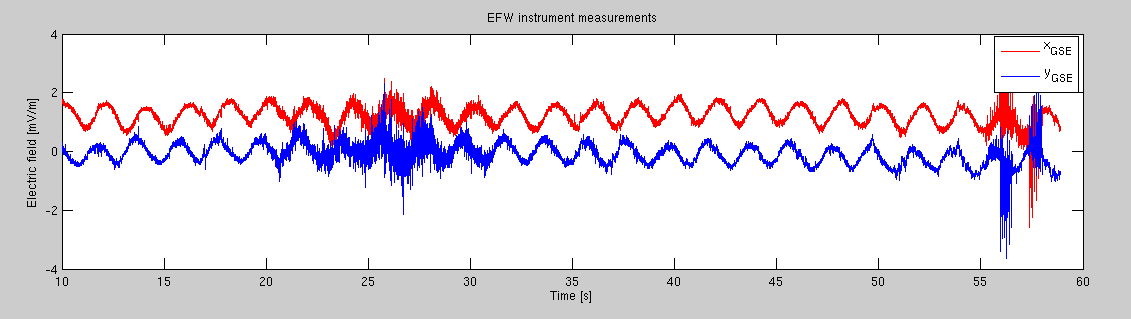
\includegraphics[width=\textwidth]{Figures/EFW_measurement.png}
\caption{EFW Measurement Data}
\label{fig:EFW}
\end{figure}

\begin{figure}[htb!]
\centering
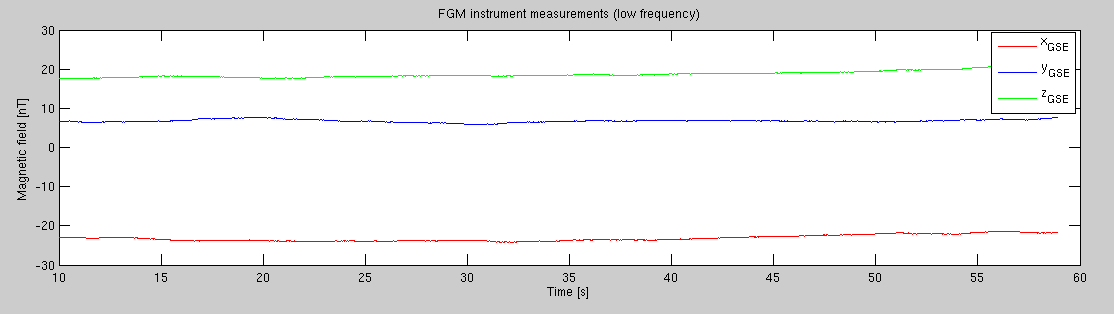
\includegraphics[width=\textwidth]{Figures/FGM_measurement.png}
\caption{FGM Measurement Data}
\label{fig:FGM}
\end{figure}

\begin{figure}[htb!]
\centering
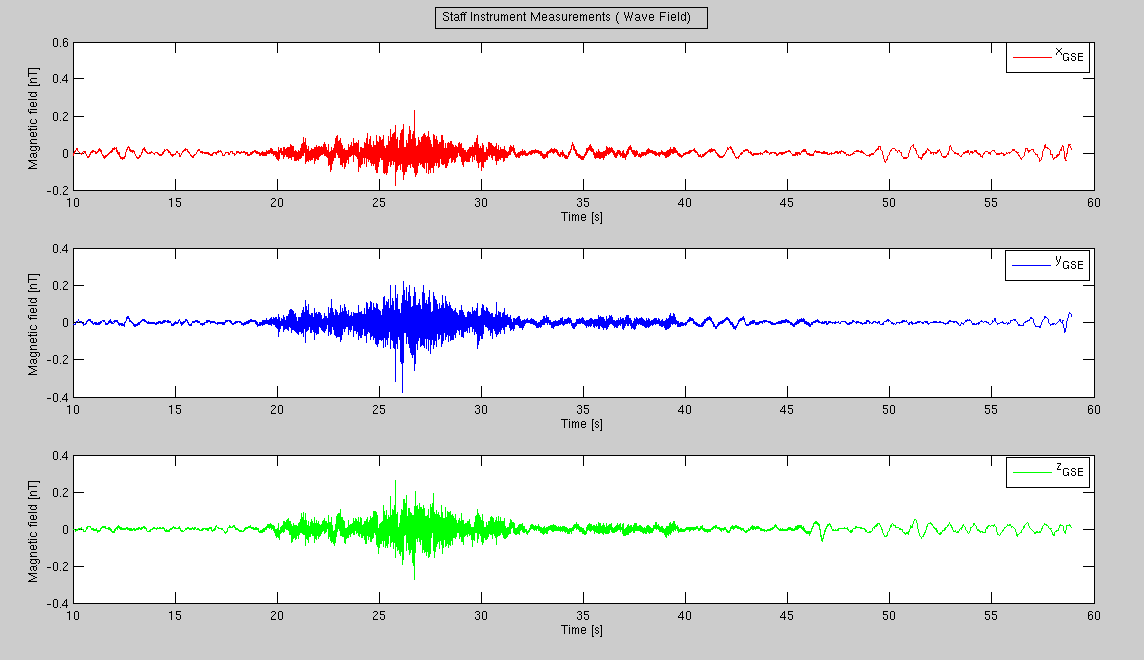
\includegraphics[width=\textwidth]{Figures/Staff_measurement.png}
\caption{Staff Instrument Measurement Data}
\label{fig:Staff}
\end{figure}

\subsection{Question 3}
\textit{Estimate the frequency of the waves by looking at the times series only. Describe how you do. What is you result?}

Roughly estimated wave period is about 0.01 s (zoomed in and estimated between 2 peaks). Frequency = 1/0.01 = 100 Hz.

\subsection{Question 4}
\textit{Compute the fundamental frequencies (electron and proton gyrofrequencies and the electron plasma frequency) in the plasma. The background magnetic field you have in the data. The density can be found from the overview data. However, the ion density is usually underestimated. Therefore, it is a good idea to compare with the high frequency emissions obtained by the WHISPER instrument. In the WHISPER data you can identify the electron plasma frequency directly, as a thin horizontal line visible most of the time. What density does the WHISPER signal correspond to? Compare the wave frequency with the fundamental frequencies. What are you conclusions?}

From overview data, ion density is $~1.5 \; cm^3$. The minimum and maximum Electron gyrofrequency are 0.82 kHz and 0.88 kHz respectively while the minimum and maximum Proton gyrofrequency is $0.45091$ Hz and $0.48342$ Hz respectively. The electron Plasma frequency is 10.9 kHz considering a density of $~1.5 \; cm^3$. The estimated plasma frequency from WHISPER is 16 kHz. This was used to calculate the electron density and a value of $n= 3.1746 \; cm^{−3}$ was obtained.


From the above results it can be concluded that only the electrons cause the wave because the wave frequency is much bigger than the proton gyrofrequency. The protons are too slow to have any effect on the appearance of this wave.


\subsection{Question 5}
\textit{Compute the PSD of the electric and magnetic wave fields for the entire time period. If you want you can use the Matlab-function PSDvsFREQ(). Compare with your results obtained in 2 and 3. Also, investigate the how the error changes when you sum over fewer records. If you want you can use the errorbar() function to visualize this. Which are your
conclusions?}\\

The Figures \ref{fig:PSD_electric} and \ref{fig:PSD_magnetic} show the PSD of electric and magnetic field respectively. The peaks are around 90-100 Hz. Which corresponds to our rough estimation in question 3. The Figures \ref{fig:PSD_electric_50} and \ref{fig:PSD_magnetic_50} show the PSD of electric and magnetic fields when fewer records have been used along with the error bars. It can bee seen the the error is increases when less records are used. The parameters used are NK=200; Kstart=1; Kshift=100;N=1024; NG=N; GW=NG/4;



\begin{figure}[htb!]
\centering
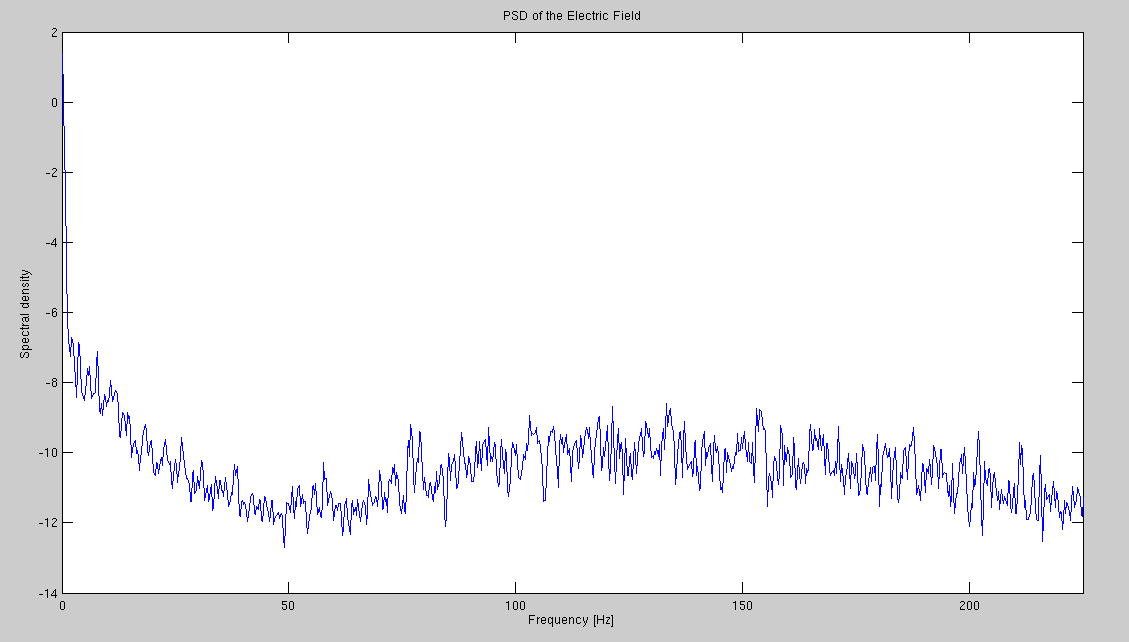
\includegraphics[width=\textwidth]{Figures/PSD_electric.png}
\caption{PSD of Electric Field with N=1024.}
\label{fig:PSD_electric}
\end{figure}

\begin{figure}[htb!]
\centering
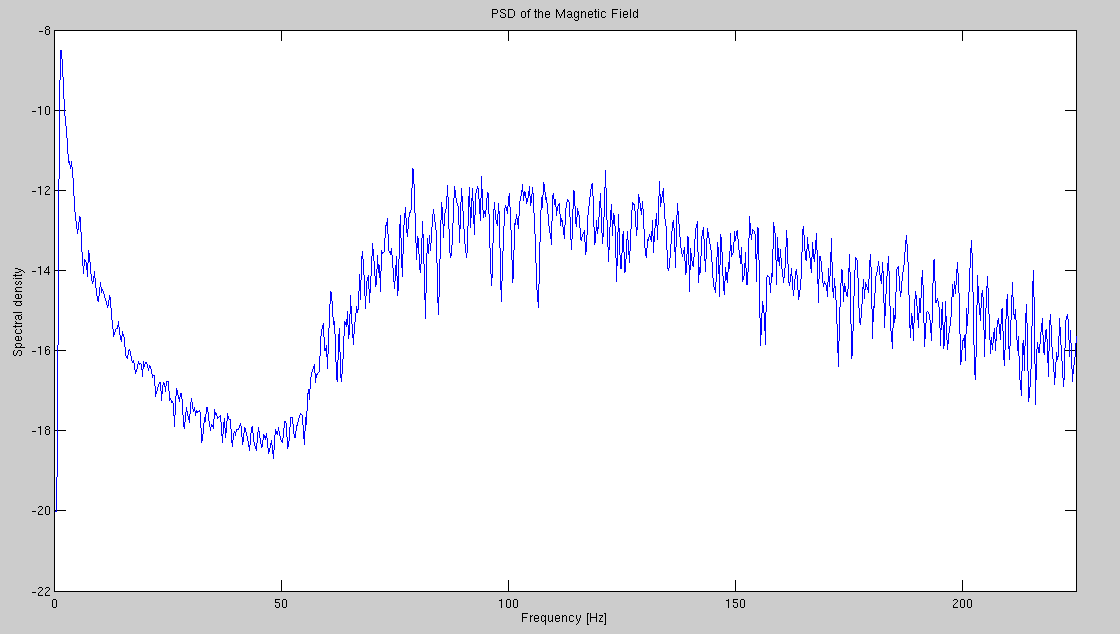
\includegraphics[width=\textwidth]{Figures/PSD_magnetic.png}
\caption{PSD of Magnetic Field with N=1024.}
\label{fig:PSD_magnetic}
\end{figure}

\begin{figure}[htb!]
\begin{minipage}[c]{0.5\linewidth}
\centering
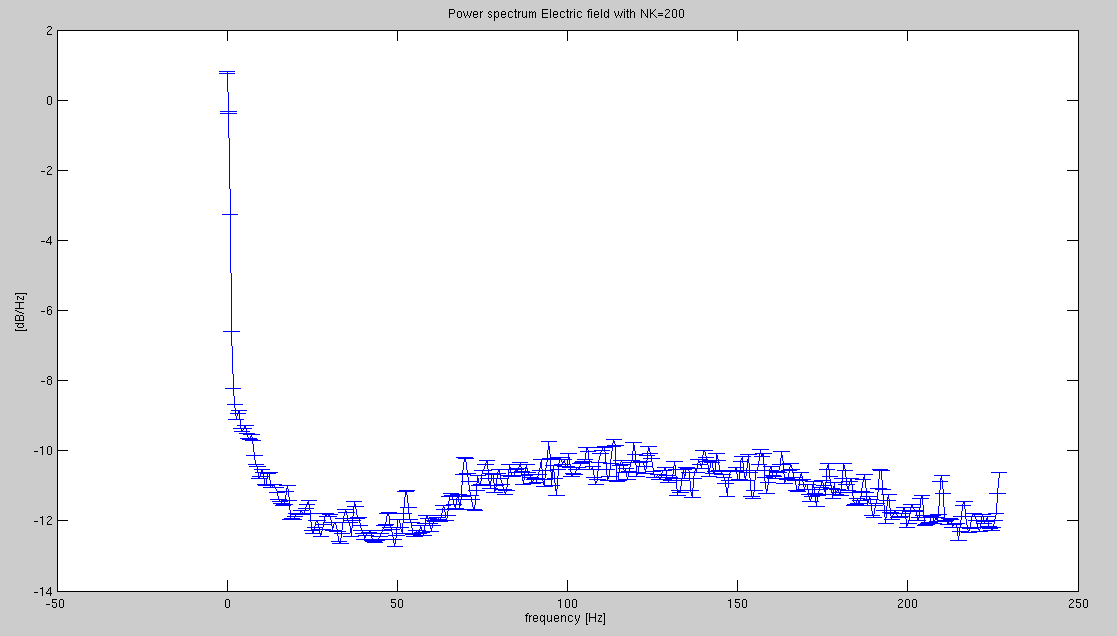
\includegraphics[width=8cm]{Figures/PSD_electric_200.png}
\caption{PSD of Electric Field Nk=200}
\label{fig:PSD_electric_200}
\end{minipage}
\hspace{0.1cm}
\begin{minipage}[c]{0.5\linewidth}
\centering
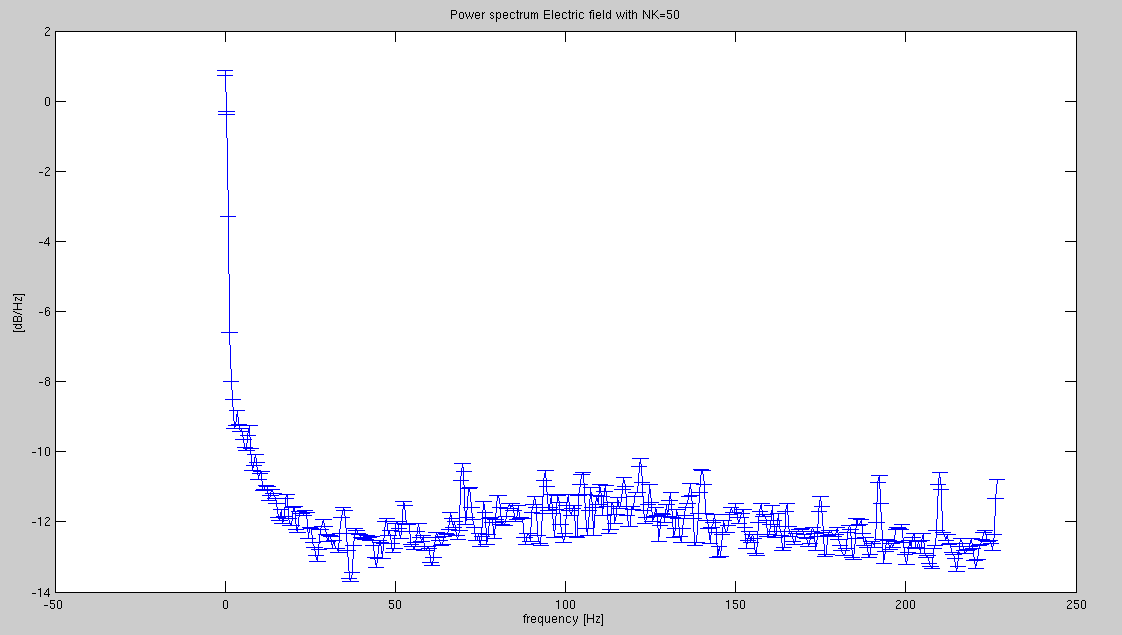
\includegraphics[width=8cm]{Figures/PSD_electric_50.png}
\caption{PSD of Electric Field Nk=50}
\label{fig:PSD_electric_50}
\end{minipage}
\end{figure}

\begin{figure}[htb!]
\begin{minipage}[c]{0.5\linewidth}
\centering
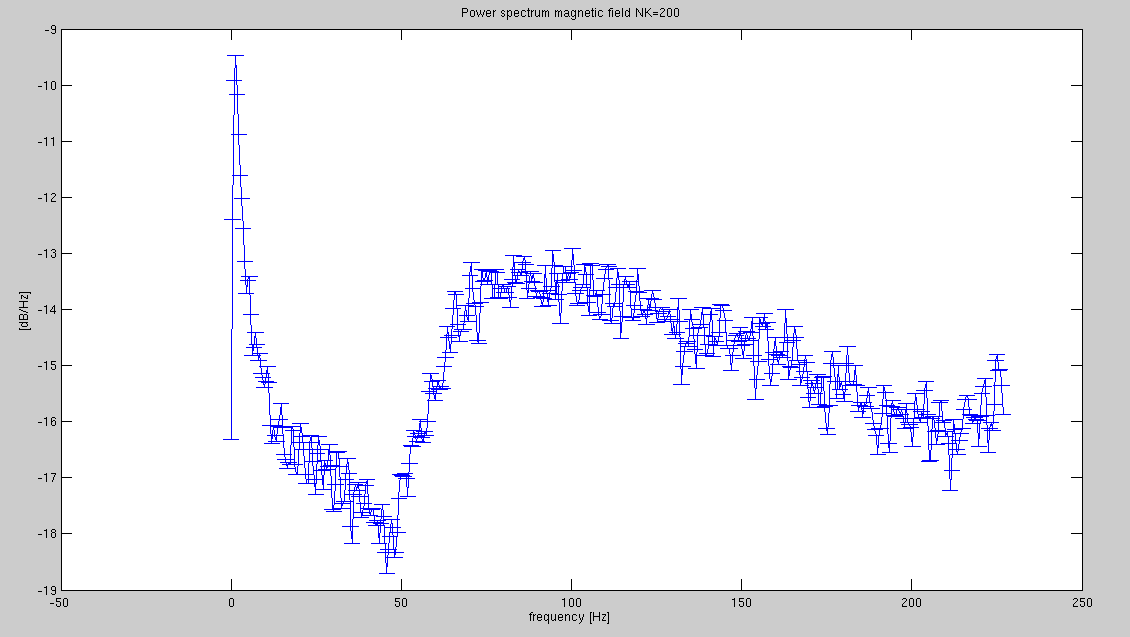
\includegraphics[width=8cm]{Figures/PSD_magnetic_200.png}
\caption{PSD of Magnetic Field Nk=200}
\label{fig:PSD_magnetic_200}
\end{minipage}
\hspace{0.1cm}
\begin{minipage}[c]{0.5\linewidth}
\centering
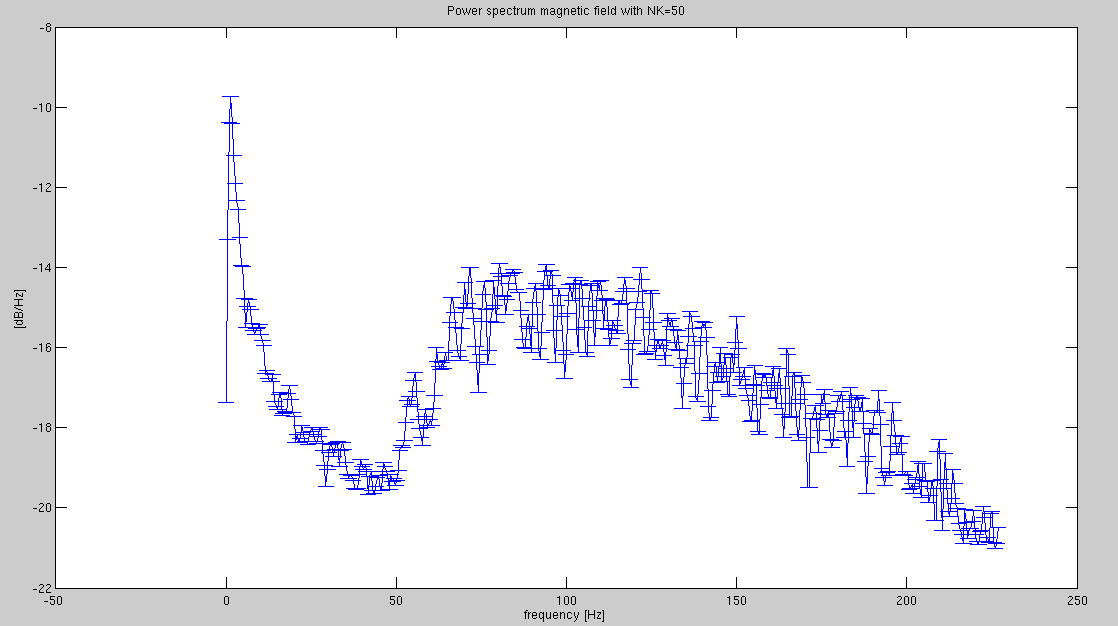
\includegraphics[width=8cm]{Figures/PSD_magnetic_50.png}
\caption{PSD of Magnetic Field Nk=50}
\label{fig:PSD_magnetic_50}
\end{minipage}
\end{figure}



\subsection{Question 6}
\textit{Look at (=make PSDs for) two different frequency ranges: 0-225 Hz and 0-2 Hz. You should aim at good statistics so the frequency resolution should be different in the two plots. The frequency resolution is given by $Δf=1/NΔt$, where Δt is the time between two samples and N is the record length used in the Fourier transform. For each of the plots: provide all the information about the PSD you present: The length of the record, the shift between records and the total number of records used.}\\

The Figures \ref{fig:PSD_electric_z_2} and \ref{fig:PSD_magnetic_z_2} show the PSD of electric and magnetic field for 0 to 2 Hz frequency. 

\begin{figure}[htb!]
\begin{minipage}[c]{0.5\linewidth}
\centering
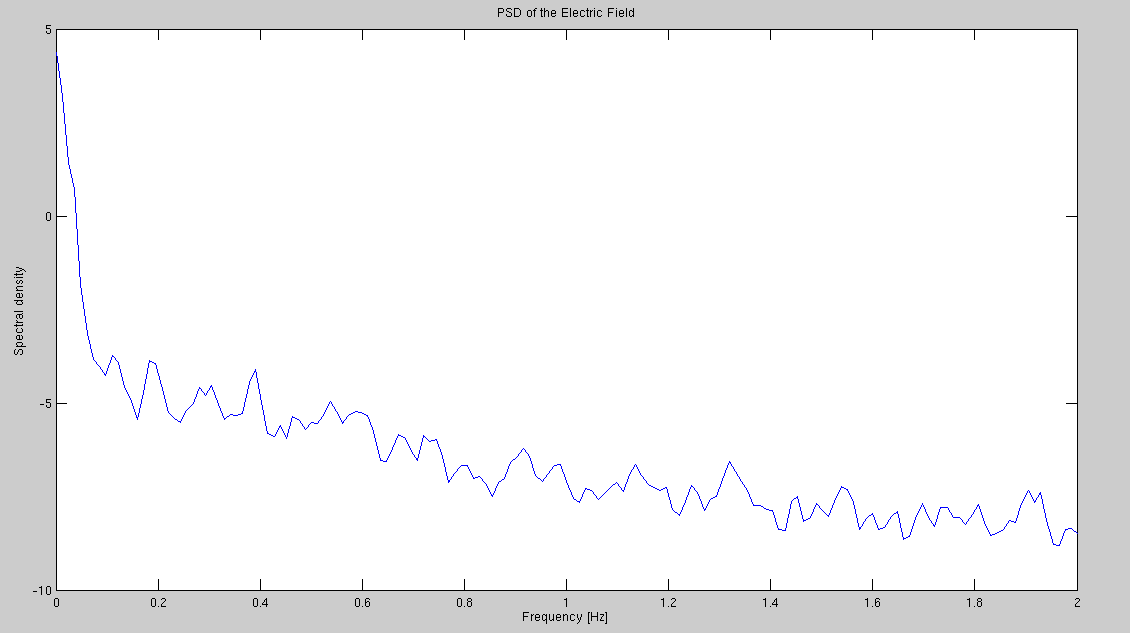
\includegraphics[width=8cm]{Figures/PSD_electric_z_2.png}
\caption{PSD of Electric Field for frequncy 0 to 2 Hz}
\label{fig:PSD_electric_z_2}
\end{minipage}
\hspace{0.1cm}
\begin{minipage}[c]{0.5\linewidth}
\centering
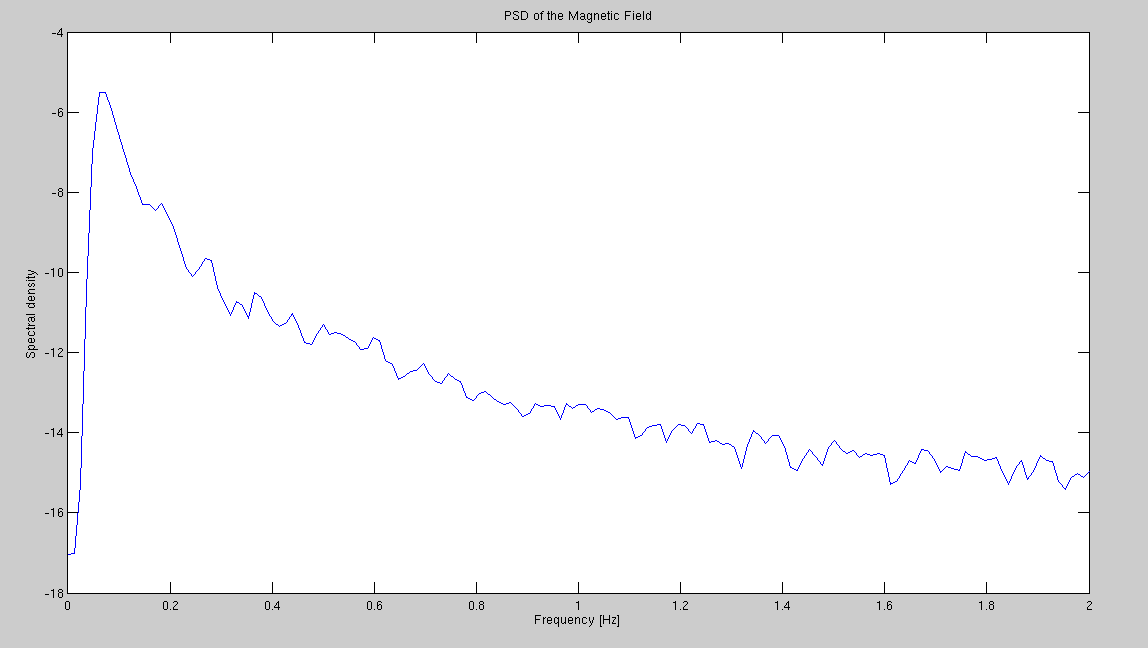
\includegraphics[width=8cm]{Figures/PSD_magnetic_z_2.png}
\caption{PSD of Magnetic Field for frequency 0 to 2 Hz}
\label{fig:PSD_magnetic_z_2}
\end{minipage}
\end{figure}

\begin{figure}[htb!]
\begin{minipage}[c]{0.5\linewidth}
\centering
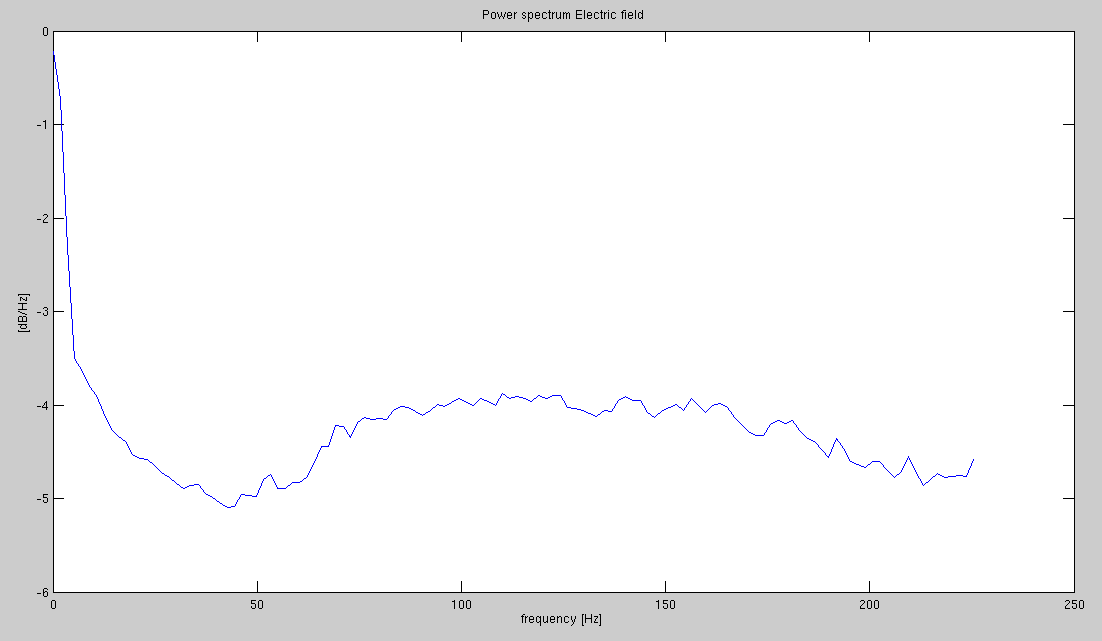
\includegraphics[width=8cm]{Figures/PSD_electric_N_256.png}
\caption{PSD of Electric Field for frequncy 0 to 225 Hz with N=256}
\label{fig:PSD_electric_N_256}
\end{minipage}
\hspace{0.1cm}
\begin{minipage}[c]{0.5\linewidth}
\centering
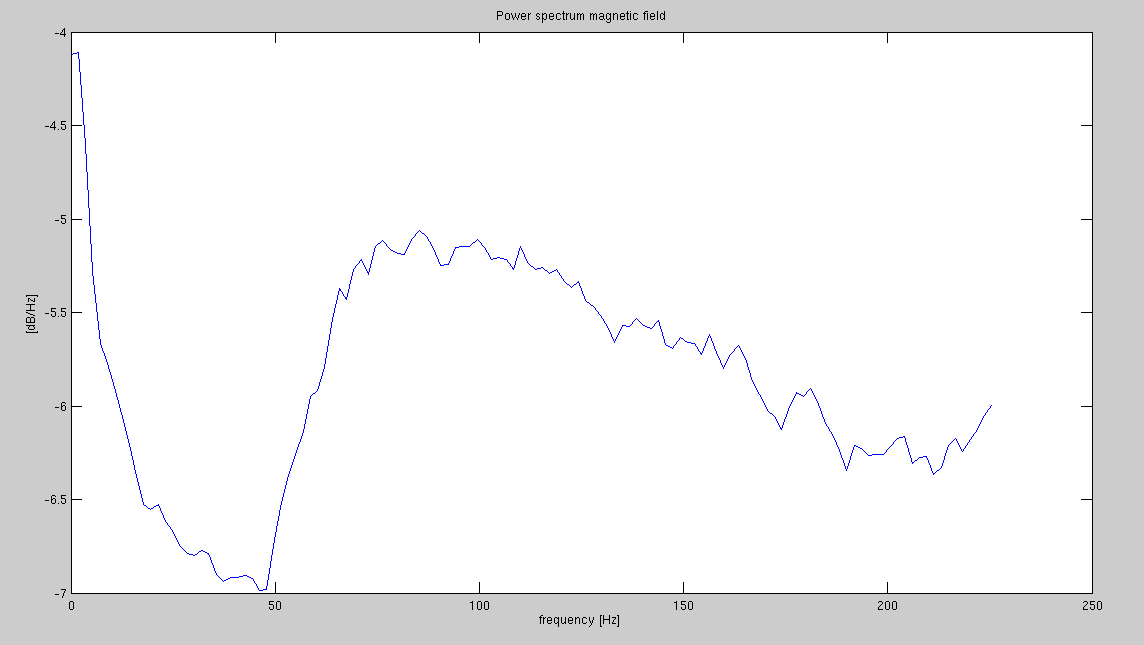
\includegraphics[width=8cm]{Figures/PSD_magnetic_N_256.png}
\caption{PSD of Magnetic Field for frequency 0 to 225 Hz with N=256}
\label{fig:PSD_magnetic_N_256}
\end{minipage}
\end{figure}


\subsection{Question 7}
\textit{Plot spectrograms (=PSD versus time and frequency) of both the electric and magnetic fields. You can do this by using the Matlab function means() and ignoring the wave vector output. Try different resolutions in time and frequency.What are you conclusions?}\\

The Figures \ref{fig:spectrogram_electric_highF} and \ref{fig:spectrogram_electric_highT} show the spectrogram of electric field with high frequency and high time resolution respectively. The Figures \ref{fig:spectrogram_magnetic_highF} and \ref{fig:spectrogram_magnetic_highT} show the spectrogram of the magnetic field with high frequency and high time resolution respectively. The time when the wave appears is clearly visible, because of the power increase with high time resolution. But the high frequency shows the wave better. So in this case high frequency has to be used. The parameters used for high frequency resolution are $$NG = 4096;N = NG;GW = N/2;Kshift = 2048;Kstart = 1;ntshift=1;ntaver=2$$The parameters used for high time resolution are $$NG = 64;N = NG;GW = N/2;Kshift = 32;Kstart = 1;ntshift=1;ntaver=2$$

\begin{figure}[htb!]
\begin{minipage}[c]{0.5\linewidth}
\centering
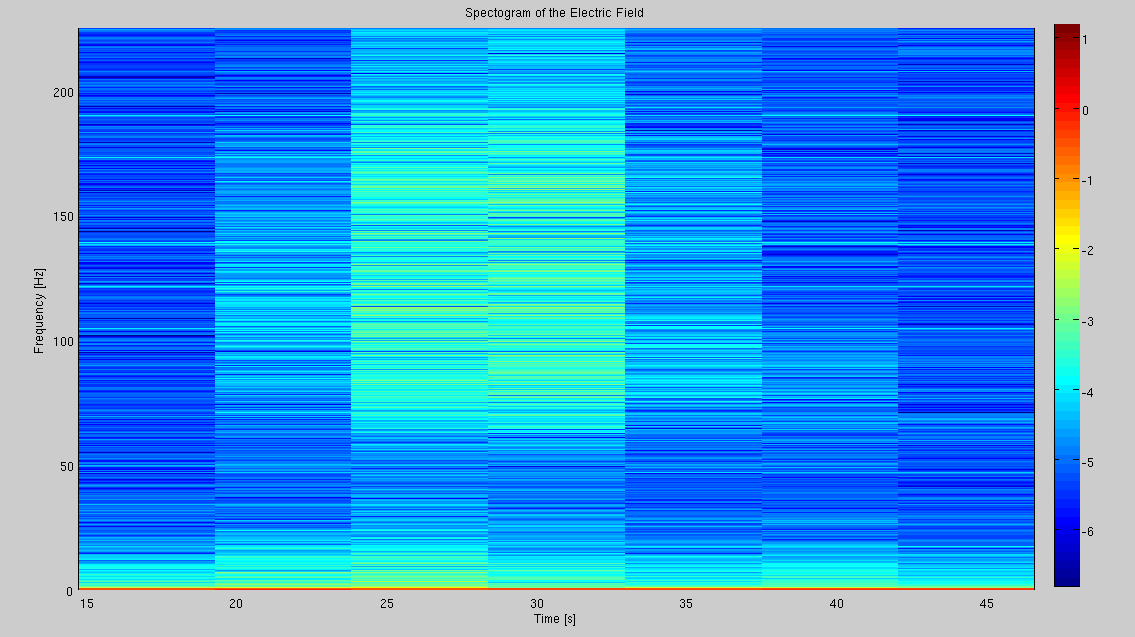
\includegraphics[width=8cm]{Figures/spectrogram_electric_highF.png}
\caption{Spectrogram of Electric Field with high frequency resolution}
\label{fig:spectrogram_electric_highF}
\end{minipage}
\hspace{0.1cm}
\begin{minipage}[c]{0.5\linewidth}
\centering
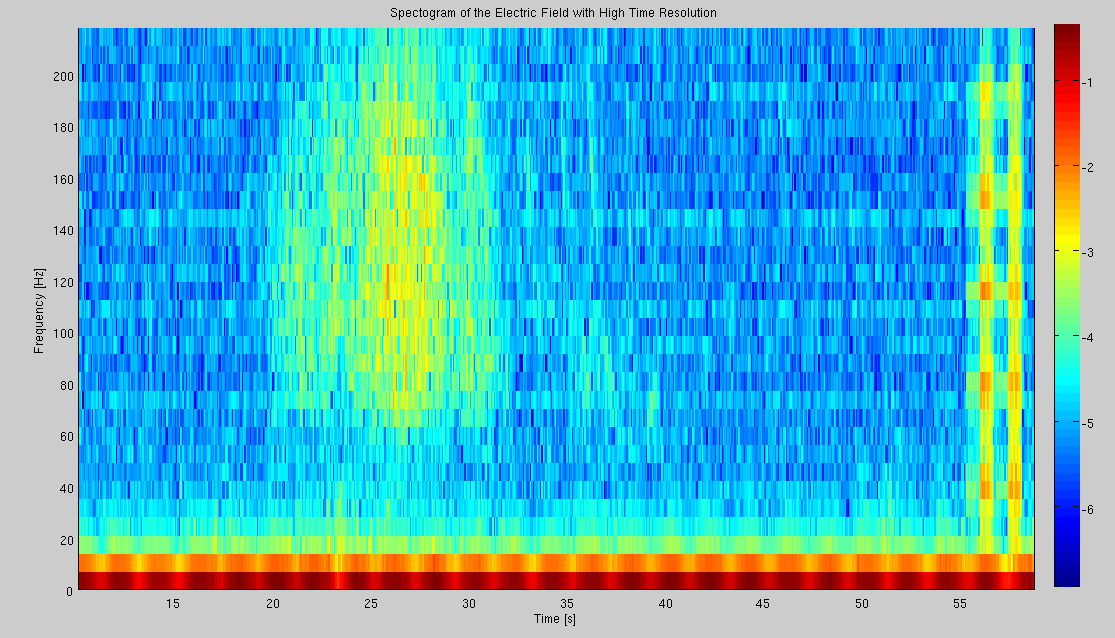
\includegraphics[width=8cm]{Figures/spectrogram_electric_highT.png}
\caption{Spectrogram of Electric Field with high time resolution}
\label{fig:spectrogram_electric_highT}
\end{minipage}
\end{figure}

\begin{figure}[htb!]
\begin{minipage}[c]{0.5\linewidth}
\centering
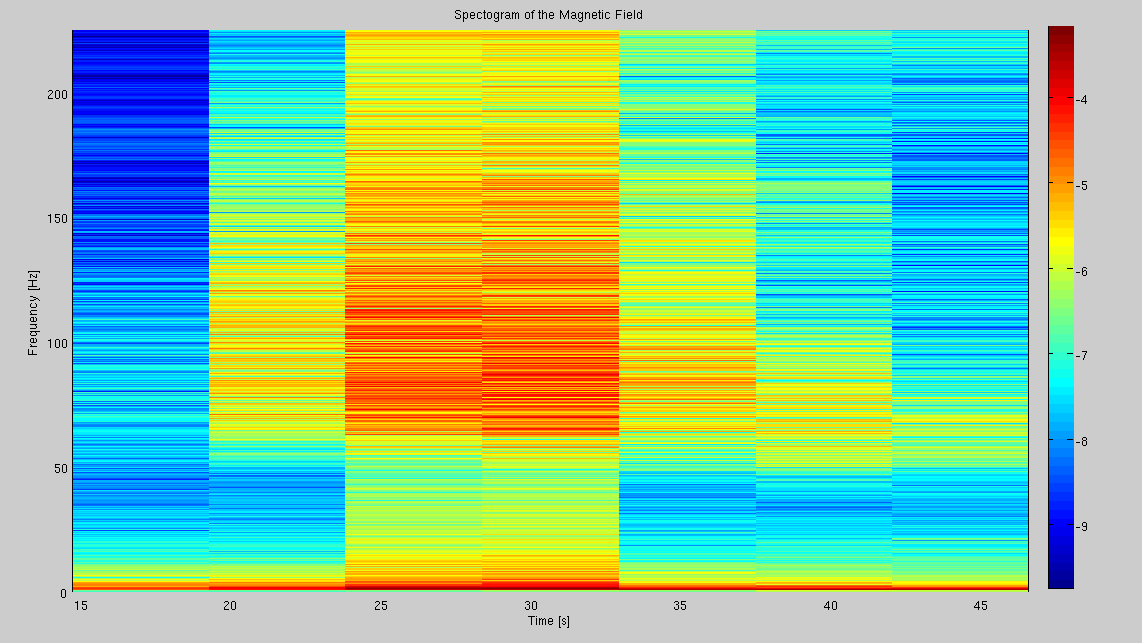
\includegraphics[width=8cm]{Figures/spectrogram_magnetic_highF.png}
\caption{Spectrogram of Magnetic Field with high frequency resolution}
\label{fig:spectrogram_magnetic_highF}
\end{minipage}
\hspace{0.1cm}
\begin{minipage}[c]{0.5\linewidth}
\centering
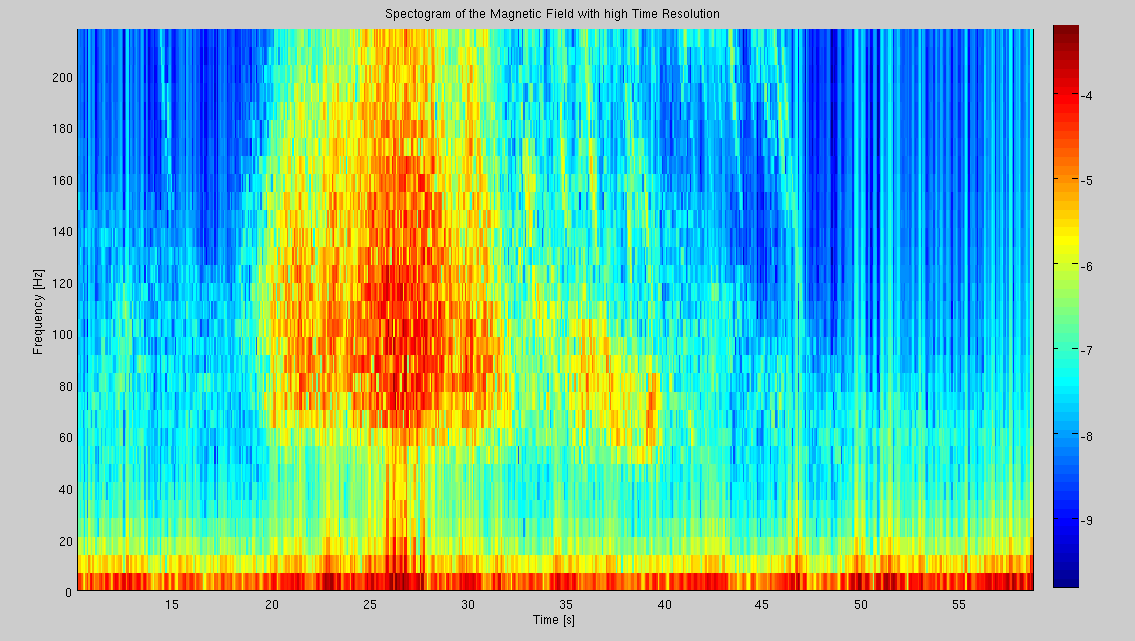
\includegraphics[width=8cm]{Figures/spectrogram_magnetic_highT.png}
\caption{Spectrogram of Magnetic Field with high time resolution}
\label{fig:spectrogram_magnetic_highT}
\end{minipage}
\end{figure}

\subsection{Question 8}
\textit{Now we can produce a so-called hodogram , which shows how the wave field vector moves in the plane perpendicular to B0. If the field vector moves in the same direction as a positive ion would gyrate then the wave is left-hand polarized. If the vector rotates in the opposite direction the wave is righthand polarized. Plot the magnetic field vector in this plane and determine the polarization of the waves. Sometimes it is easier to see the rotation if you normalize the length of the vectors to 1. Do the same with the electric field wave vector.}\\

The Figures \ref{fig:hodogram_electric} and \ref{fig:hodogram_magnetic} show the hodogram for the electric and magnetic field respectively. It starts with red then green and blue. The hodogrom of magnetic field seems to moving in counter-clock wise direction and hence the magnetic field is right hand polarized. The electric field seems to move in the counter clock wise direction, so it might accelerate electrons and slow down ions.

\begin{figure}[hbt!]
\begin{minipage}[c]{0.5\linewidth}
\centering
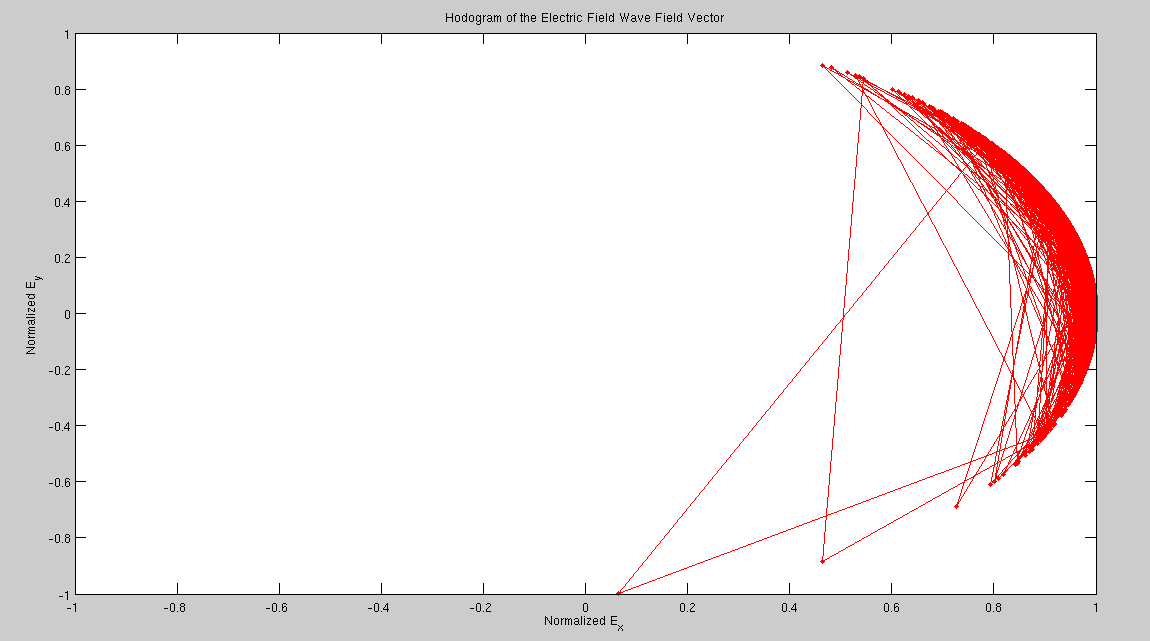
\includegraphics[width=8cm]{Figures/hodogram_electric.png}
\caption{Hodogram of Electric Field.}
\label{fig:hodogram_electric}
\end{minipage}
\hspace{0.1cm}
\begin{minipage}[c]{0.5\linewidth}
\centering
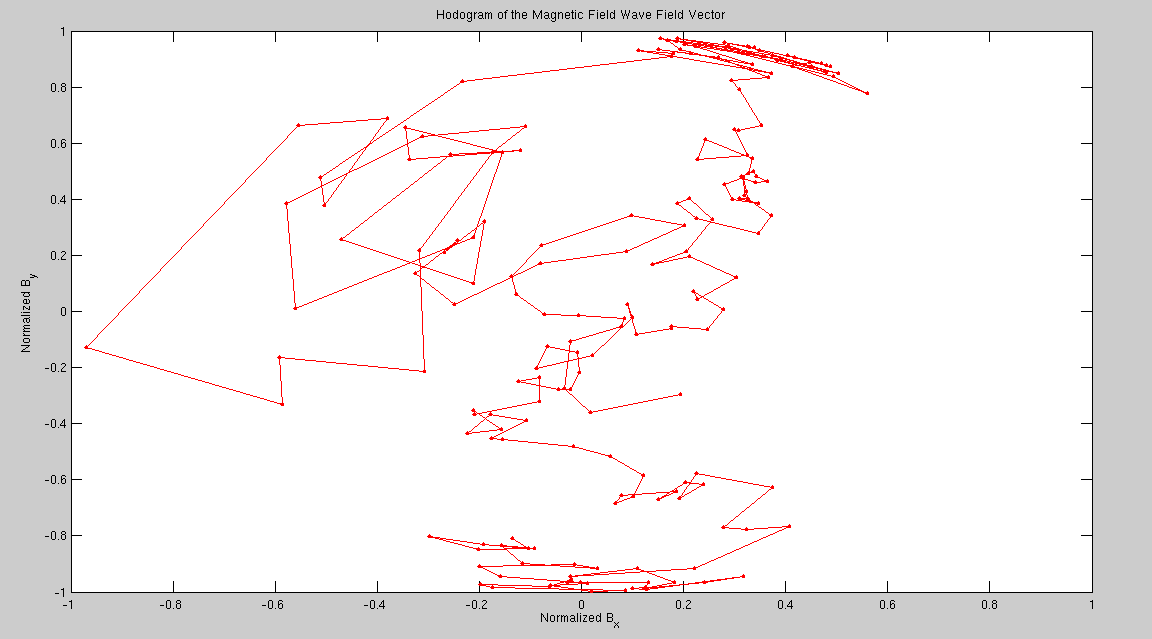
\includegraphics[width=8cm]{Figures/hodogram_magnetic.png}
\caption{Hodogram of Magnetic Field}
\label{fig:hodogram_magnetic}
\end{minipage}
\end{figure}

\clearpage
%----------------------------------------------------------------------------------------
%	SECTION 2. PARTICLE MEASUREMENTS
%----------------------------------------------------------------------------------------
\section{Particle Measurements}

For this part of the practical we have been provided the particle data from the SWIM
instrument onboard the Chandrayaan-1 spacecraft. Chandrayaan-1 orbits the moon at an altitude of 100 km. The position of the spacecraft at different times is shown in the Figures \ref{fig:orbit_1069} and \ref{fig:orbit_1070}, which also show the position of the moon with respect to Earth.\cite{Stenberg:2012_2b}

\begin{figure}[htb!]
\begin{minipage}[c]{0.5\linewidth}
\centering
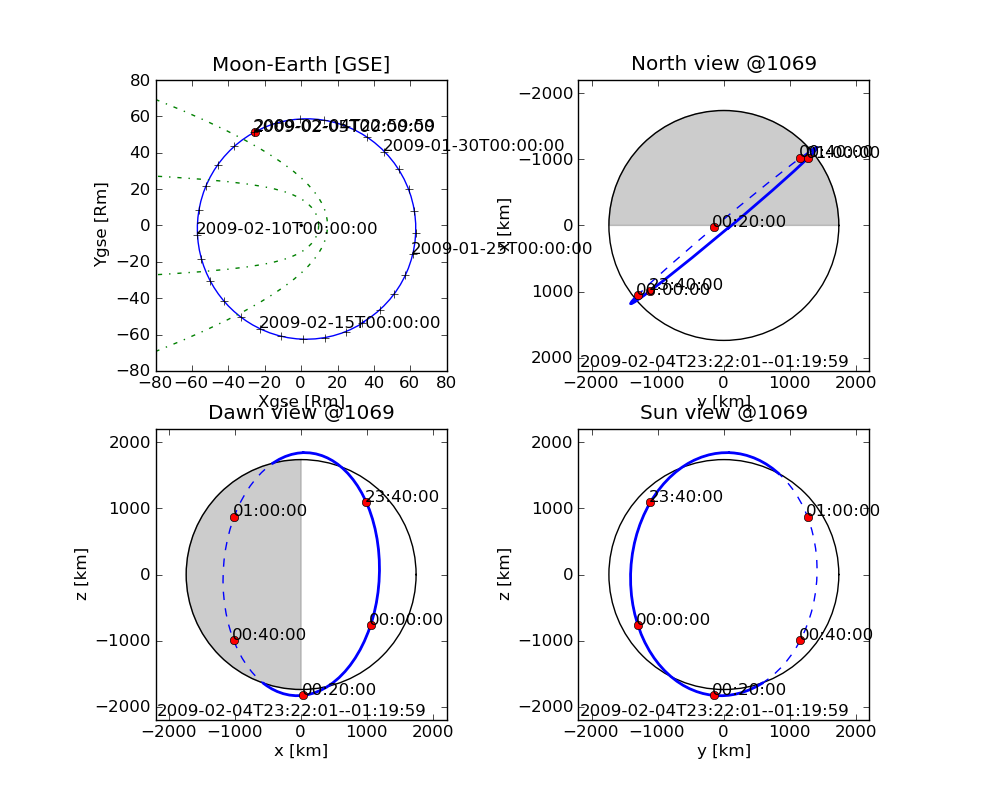
\includegraphics[width=9cm]{Figures/orbit_1069.png}
\caption{Position of the instrument in Orbit 1069}
\label{fig:orbit_1069}
\end{minipage}
\hspace{0.2cm}
\begin{minipage}[c]{0.5\linewidth}
\centering
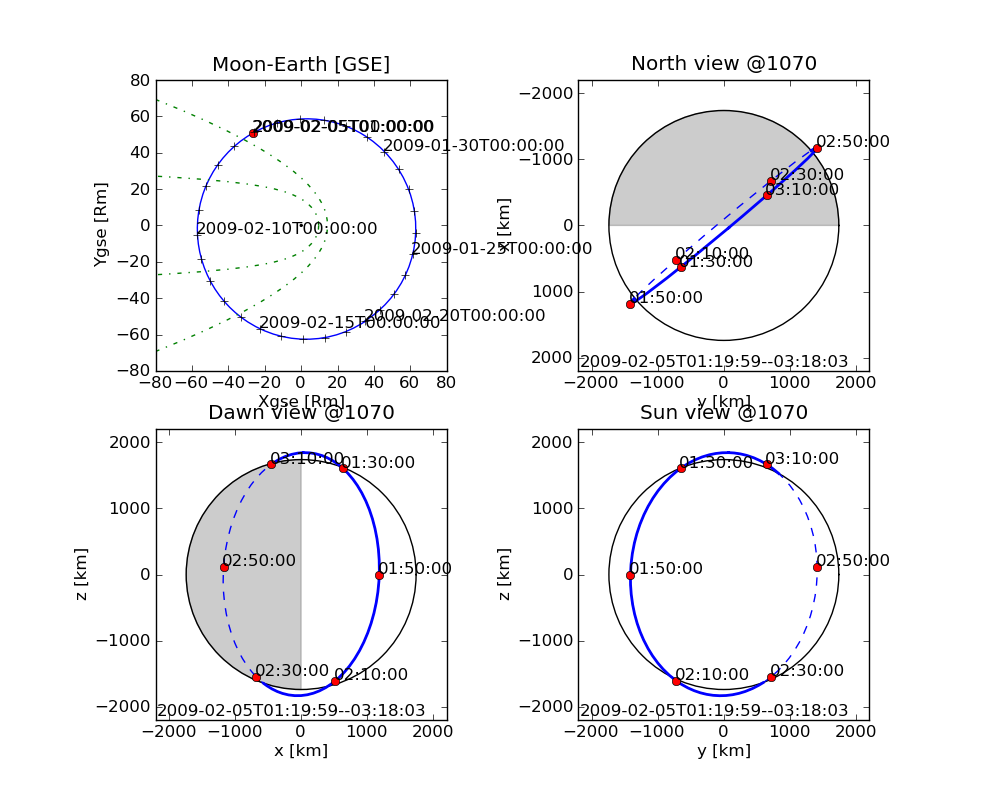
\includegraphics[width=9cm]{Figures/orbit_1070.png}
\caption{Position of the instrument in Orbit 1070}
\label{fig:orbit_1070}
\end{minipage}
\end{figure}


\subsection{Question 1}
\textit{Plot spectrograms, that is, the number of counts versus time and energy, for the
two orbits. The different energy levels you find in a comment line in the data files.
Once every orbit SWIM looks at the solar wind. Identify when this happens in the two
orbits.}

The spectrograms for the orbits 1069 and 1070 is shown in Figure \ref{fig:spectrogram_1069} and \ref{fig:spectrogram_1070} respectively. When SWIM looks at the solar wind the number of solar wind particles that hit the instrument increases significantly which is observable as the red portion in Figures \ref{fig:spectrogram_1069} and \ref{fig:spectrogram_1070}. For orbit 1069, it occurs approximately between $100th$ and $350th$ observation time bin which corresponds to UTC 05:29 to UTC 06:02 hours. For orbit 1070, it occurs approximately between $25th$ and $250th$ observation time bin which corresponds to UTC 07:22 to UTC 08:12 hours.

\begin{figure}[htb!]
\centering
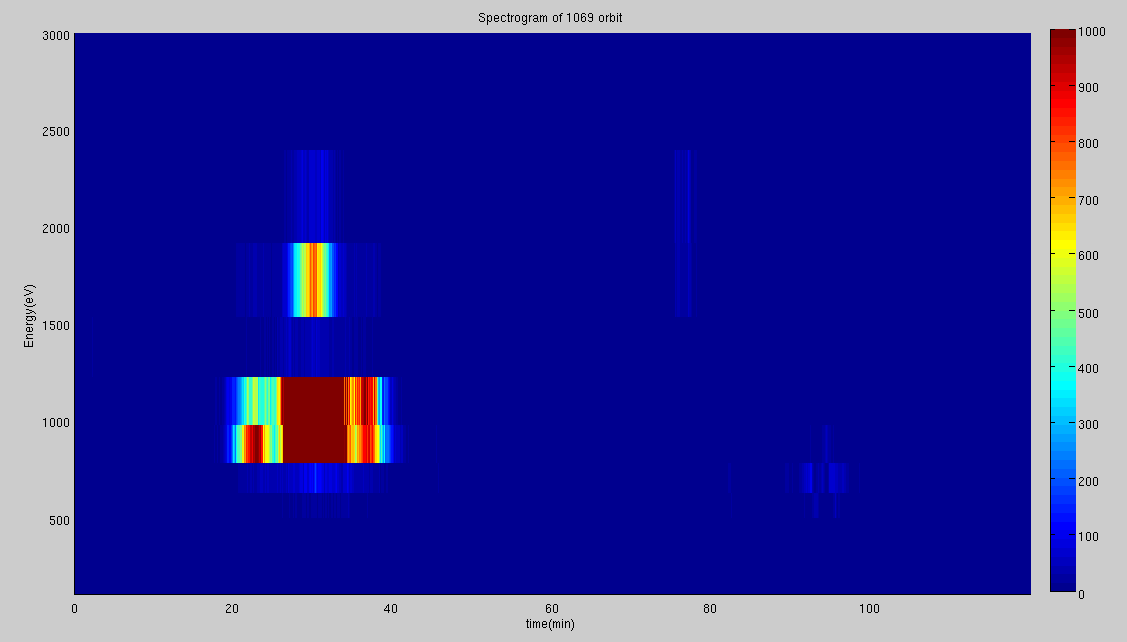
\includegraphics[scale=0.35]{Figures/spectrogram_1069.png}
\caption{Spectrogram of the 1069 Orbit}
\label{fig:spectrogram_1069}
\end{figure}

\begin{figure}[htb!]
\centering
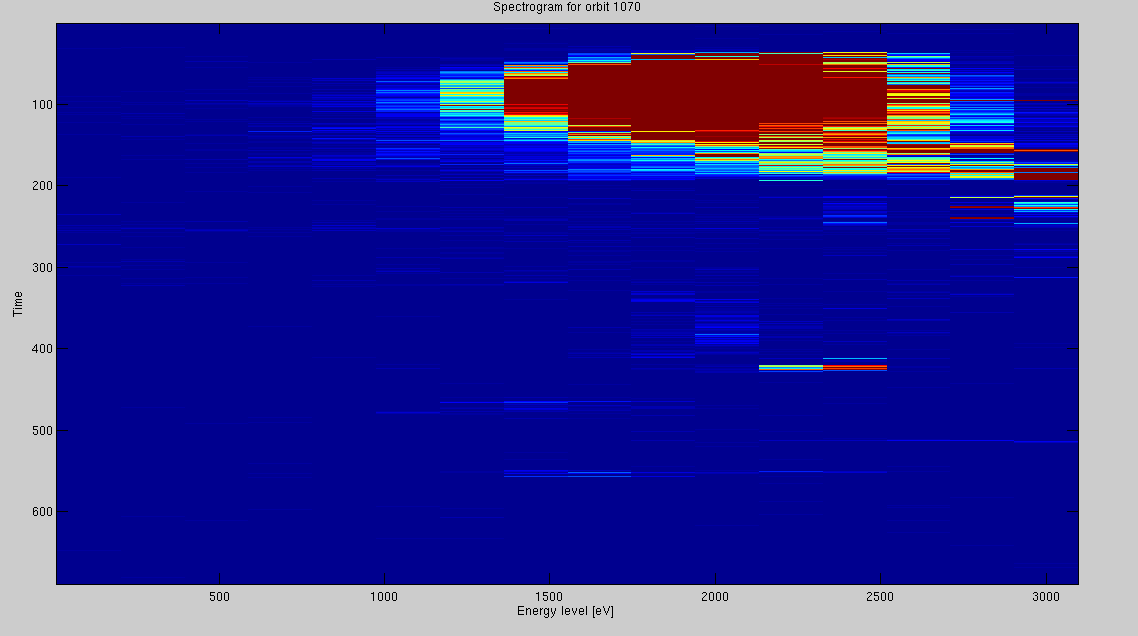
\includegraphics[scale=0.35]{Figures/spectrogram_1070.png}
\caption{Spectrogram of the 1070 Orbit}
\label{fig:spectrogram_1070}
\end{figure}

\subsection{Question 2}
\textit{Protons are the main ions in the solar wind, but can you identify any other
components? Motivate you answer!}

In Figure \ref{fig:spectrogram_1069} we observe two counts in two color areas one red and one light blue that correspond to different energy levels this suggest that there are two different components. The larger coloured area corresponds to protons because they are the main constituent of solar wind. The other energy colour could be because of Helium ions. Helium has a higher energy because all the solar wind particles move with the same velocity and helium has four times the mass of a proton and twice its charge so Helion ions have more energy.

\subsection{Question 3}
\textit{Make energy spectra, this is, plot observed counts versus energy for a selected
time interval around the solar wind observation.}

The energy spectra for the time when the SWIM instrument looks at the solar wind for the orbit 1069 and orbit 1070 is shown in Figure \ref{fig:energy_spectra_1069} and \ref{fig:energy_spectra_1070} respectively

\begin{figure}[htb!]
\centering
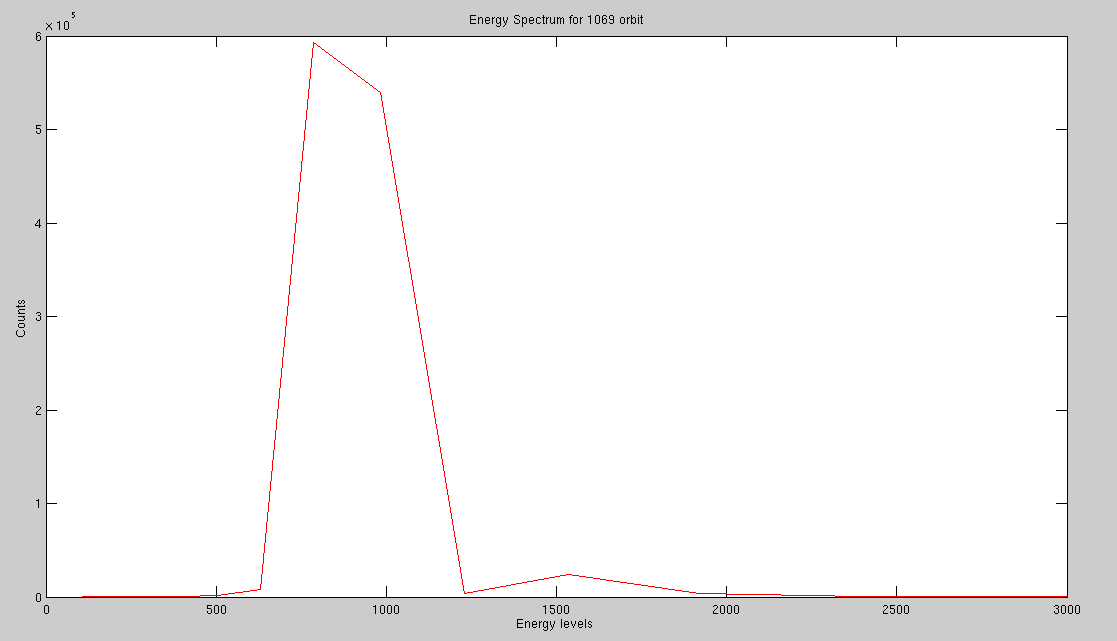
\includegraphics[scale = 0.35]{Figures/energy_spectra_1069.png}
\caption{Energy Spectra of the 1069 Orbit}
\label{fig:energy_spectra_1069}
\end{figure}

\begin{figure}[htb!]
\centering
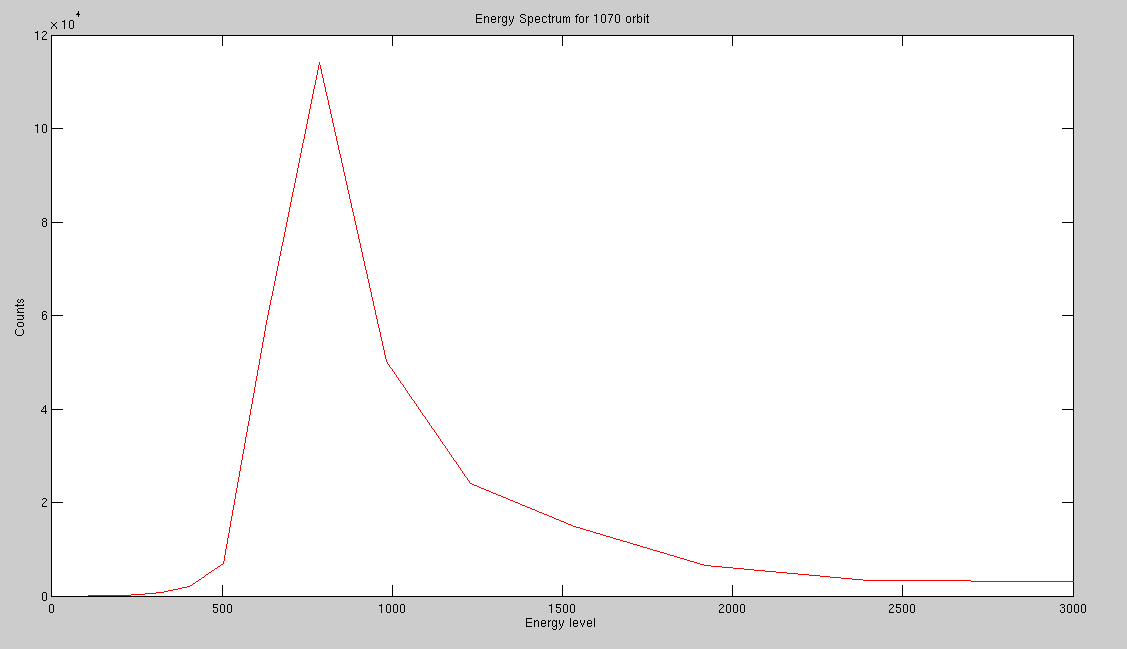
\includegraphics[scale = 0.35]{Figures/energy_spectra_1070.png}
\caption{Energy Spectra of the 1070 Orbit}
\label{fig:energy_spectra_1070}
\end{figure}

\subsection{Question 4}
\textit{Determine the solar wind proton velocity and temperature by first transforming the
data from energy to velocity space and then fitting a Maxwellian distribution. What
temperatures and velocities do you get? Are there differences between the orbits? If
so, why?}\\

For the orbit 1070 the proton velocity is 389.4 $Km/s$ and temperature is $T= 1.645 \times 10^5 K$ 
and for the orbit 1069 the proton velocityis 410.1 $Km/s$ and the temperature is  $T = 4.944 \times 10^4 K $. The differences between the two orbits are relatively small and could be because of the variable nature of the solar wind.


\subsection{Question 5}
\textit{How do you determine the velocity of other components in the solar wind? What
results do you get?}\\

The SWIM instrument measures the $ \frac{E}{q}$ value and this value will be different based
on the analyzed element and will depend entirely on the mass and charge. The other component of solar winid is ionized Helium, which has four times the amount of mass as a proton. So to calculate the velocity we need to know the energy value. The $ \frac{E}{q}$ is estimated from Figure \ref{fig:spectrogram_1069} as 1550 eV. The $mass = 4*m_p$ and the charge for an ionized Helium is
$q=2 \times 1.6 \times 10^{-19}$. To calculate the energy you just take the $ \frac{E}{q}$ and multiply it with the charge.You could then determine the velocity through the kinetic energy formula $ E = \frac{mv^2}{2}$. This gives us a velocity for the Helium around 385.321 km/s


\begin{figure}[!htb]
\centering
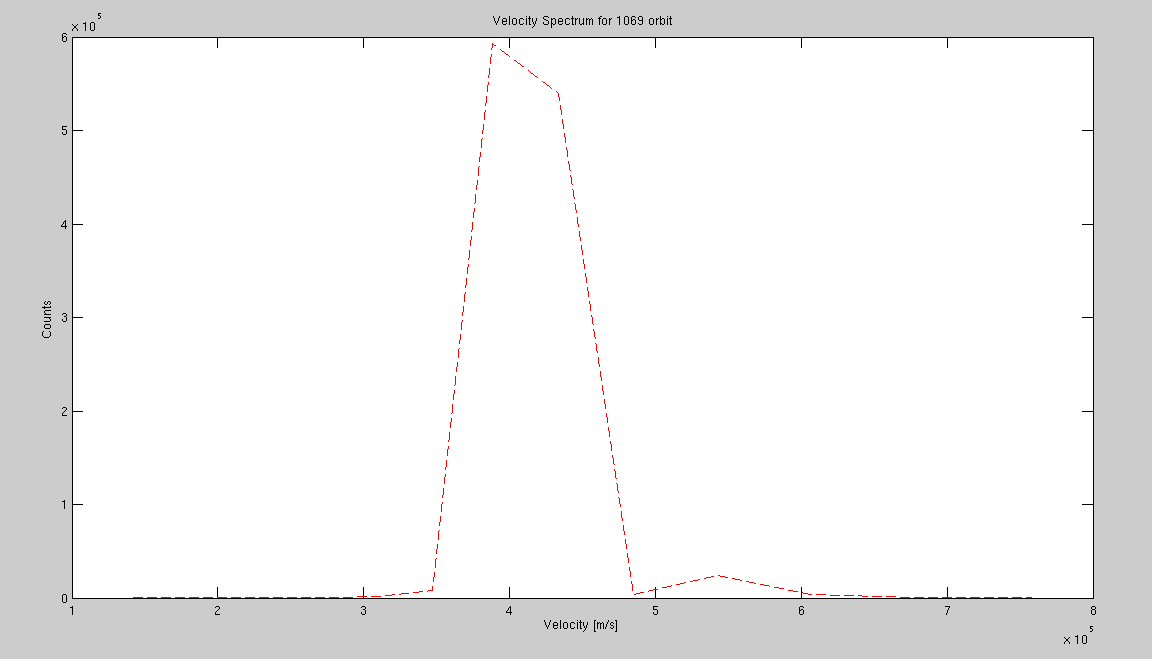
\includegraphics[scale=0.35]{Figures/velocity_spectra_1069.png}
\caption{Velocity Spectra of the 1069 Orbit}
\label{fig:Velocity_spectra_1069}
\end{figure}

\begin{figure}[htb!]
\centering
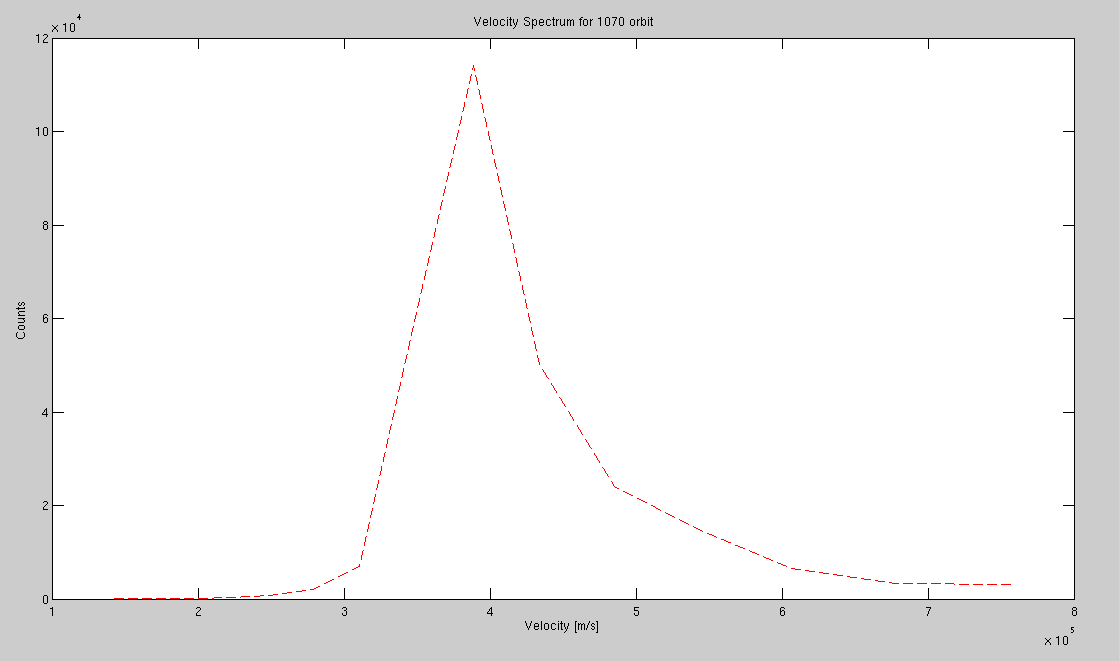
\includegraphics[scale=0.35]{Figures/velocity_spectra_1070.png}
\caption{Velocity Spectra of the 1070 Orbit}
\label{fig:Velocity_spectra_1070}
\end{figure}

\begin{figure}[!htb]
\centering
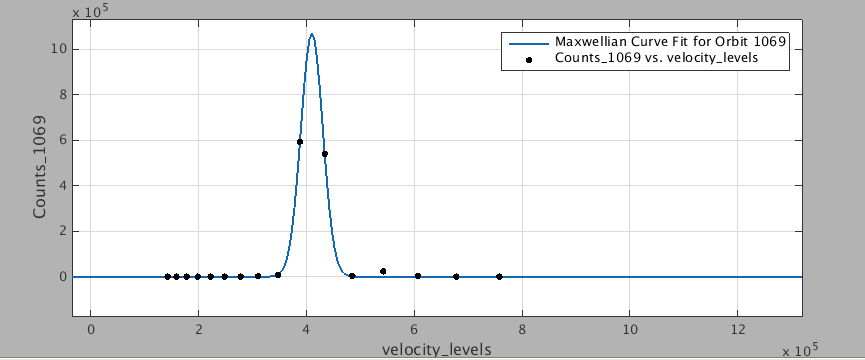
\includegraphics[scale=0.45]{Figures/curvefit_1069.png}
\caption{Maxwellian Curve fit for data from Orbit 1069}
\label{fig:curvefit_1069}
\end{figure}

\begin{figure}
\centering
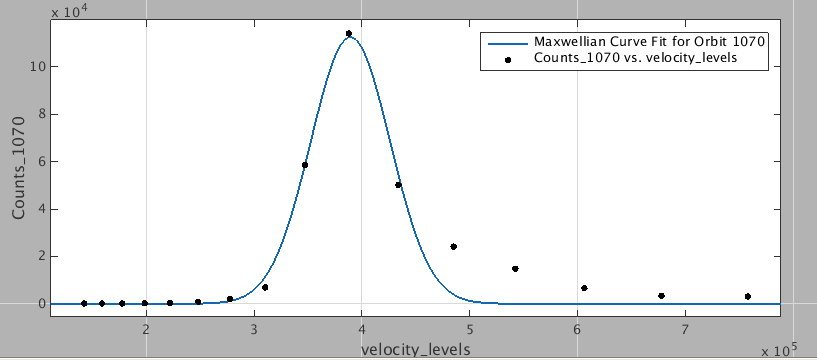
\includegraphics[scale= 0.45]{Figures/curvefit_1070.png}
\caption{Maxwellian Curve fit for data from Orbit 1070}
\label{fig:curvefit_1070}
\end{figure}

\subsection{Question 6}
\textit{Compare your results with the observations made by one of the spacecrafts ACE or WIND: \url{http://www.srl.caltech.edu/ACE/ASC/level2/lvl2DATA_SWEPAM.html} or \url{ftp://space.mit.edu/pub/plasma/wind/kp_files/}. Note that the ACE/WIND measurements are made far upstream of the spacecraft so you have to compensate for this when you compare.}\\


ACE is not at the same position as Chandrayaan-1 so we need to take the distance between ACE and Chandrayaan-1's position while making comparison between the data from both. The approximate distance is $1.5\times10^6$ km. The solar wind’s velocity is approximately 400 km/s and this means that it takes the solar wind about one hour to travel from ACE to Chandrayaan-1. So in order to compare the data between the two the data from ACE has been taken one hour before the data in Chandrayaan-1.
Data was observed from the ACE instrument from their website relating to the time of orbit 1069 and orbit 1070. It was given to be
\begin{itemize}
\item {For orbit 1069- Velocity of Solar wind was $331 Km/s$}
\item {For orbit 1070- Velocity of Solar wind was $328 Km/s$}
\end{itemize}

This is the same order of magnitude as calcuated in the previous questions.

	
\clearpage


%----------------------------------------------------------------------------------------
%	SECTION 4. REFERENCES
%----------------------------------------------------------------------------------------
\newpage
\begin{thebibliography}{9}

\bibitem{ACE:measurements}
ACE SWEPAM Level 2 Data.
\newblock {\em Measurements from the satellite ACE}.
\newblock {\url{http://www.srl.caltech.edu/ACE/ASC/level2/lvl2DATA_SWEPAM.html}}.

\bibitem{Stenberg:2012_2b}
Stenberg G.  (2012).
\newblock {\em Practical 2B. Data Analysis}.
\newblock Lule\aa \ University of Technology, Kiruna, Sweden.

\end{thebibliography}


\end{document}